% This is LLNCS.DEM the demonstration file of
% the LaTeX macro package from Springer-Verlag
% for Lecture Notes in Computer Science,
% version 2.4 for LaTeX2e as of 16. April 2010
%
\documentclass{llncs}
%
\usepackage[portuguese]{babel}
\usepackage[utf8]{inputenc}
\usepackage{makeidx}  % allows for indexgeneration
\usepackage{graphicx}
\setcounter{secnumdepth}{3}
\graphicspath{ {./img/} }
%

\begin{document}

%
\frontmatter          % for the preliminaries
%
\pagestyle{headings}  % switches on printing of running heads
%
\title{Ano Escolar}
\subtitle{Resolução de Problemas de Desisão utilizando\\
Programação em Lógica com Restrições}
%
\titlerunning{Ano Escola}  % abbreviated title (for running head)
%                                     also used for the TOC unless
%                                     \toctitle is used
%
\author{Daviz Azevedo \and João Ferreira}
%
\authorrunning{Daviz Azevedo \and João Ferreira} % abbreviated author list (for running head)
%
\institute{Faculdade de Engenharia da Universidade do Porto\\
Rua Roberto Frias, sn, 4200-465 Porto, Portugal}

\maketitle              % typeset the title of the contribution

\begin{abstract} %

O objetivo deste trabalho é a criação de um programa, em Programação em Lógica com Restrições, capaz de marcar trabalhos de casa e testes para um dado ano, restritos a certas condições.

Ao longo deste documento será descrito o desenvolvimento do trabalho realizado e os resultados obtidos.

\end{abstract}
%
\section{Introdução}
%
Devido à complexidade combinatória existente no planeamento de um Ano Escolar, é necessária uma solução optima que permita obter da melhor forma um plano de aulas ágil e eficaz.

Este trabalho tem como objetivo, para um dado Ano Escolar, marcar os trabalhos de casa e os testes para diferentes turmas e disciplinas, dependendo de variáveis definidas pelo utilizador.
Neste documento está descrito detalhadamente o problema, uma abordagem de resolução do problema e uma análise sobre a mesma. Também será discutida a estratégia de pesquisa, os predicados de visualização e filamente uma conclusão geral sobre o trabalho.


\section{Descrição do Problema}
%
O problema de otimização escolhido foi o Ano Escolar, neste problema é proposto que, o programa desenvolvido , seja capaz de marcar trabalhos de casa e testes para um número indefinido de turmas e de semanas. Em relação aos trabalhos de casa, para cada turma existe um dia livre e o número de TPC só pode ser metade do número de ocorrências da disciplina não podendo existir mais que um número determinado de TPC's no mesmo dia. Em relação aos testes, cada disciplina tem dois testes, decorrendo num número de semanas especifico (meio e fim do período) e o número máximo de testes é dois por semana, sendo que não existem testes em dias consecutivos.

\section{Abordagem}
%
Num primeiro ato de abordagem ao problema, o problema foi dividido em dois subproblemas, a marcação dos trabalhos de casa e a marcação dos testes. 

Para a marcação dos trabalhos de casa, foram realizados dois perdicados que resolvem o problema de dois pontos de vista diferente.

Para o primeiro predicado dos trabalhos de casa, foi utilizada uma estrutura de modo a limitar as variáveis utilizadas por disciplina, foi criada uma lista que contém os dias da semana, cada dia contem listas por disciplina com comprimento igual ao número de semanas para indicar, em que semanas existem ou não TPCs, naquela disciplina, daquele dia da semana. A razão pela qual foi optada esta  estrutura, foi numa tentativa de otimizar o espaço para representar os dias em que é possivél marcar trabalhos de casa para certa disciplina.
\newline

Para o segundo predicado dos trabalhos de casa, foi utilizada uma lista, onde cada index, indica a disciplina, e o elemento contido nesse index é um array de tamanho igual ao número de ocorrências dessa disciplina, ao longo do período de aulas. Esta estrutura permite ter em atenção a totalidade de ocorrências de uma dada disciplina, permitindo distribuir de melhor forma os trabalhos de casa.

Descrever com detalhe o problema de otimização ou decisão em análise.

\subsection{Variáveis de Decisão}


Em relação aos trabalhos de casa, as variáveis de decisão são: 

Para o primeiro predicado:
\begin{enumerate}
\item Dia Livre de Domínio [1,5], que representa um dos dias úteis da semana.
\item Lista de TPCs por disciplina de Domínio[0,1], que representa se existe ou não trabalho de casa em determinada semana, determinada pela sua posição.
\end{enumerate}

A lista de TPCs por disciplina, é um conceito simples, mas ligeiramente difícil de explicar, como foi descrito na secção anterior, cada disciplina de um determinado dia, tem associada uma lista, de tamanho igual ao número de semanas de aulas, em que cada posição da lista representa o número da semana e o seu conteúdo indica se existe ou não trabalho de casa, 1 em caso positivo 0 em caso negativo.


Para o segundo predicado:
\begin{enumerate}
\item Dia Livre de Domínio [1,5], que representa um dos dias úteis da semana.
\item Lista de Dias com TPC por disciplina de Domínio[0, DiasSemana ], que representa os dias em que existe trabalhos de casa, um valor maior que zero indica o dia do TPC.
\end{enumerate}



Descrever as variáveis de decisão e os seus domínios.

\subsection{Restrições}
Na prespetiva dos trabalhos de casa, as restrições aplicadas são:

Para o primeiro predicado:
\begin{enumerate}
\item Para cada disciplina de um determinado dia, o número de trabalhos de casa tem que ser igual à metade do número de semanas de aulas.

Utilizando a estrutura descrita nas últimas secções, esta restrição faz-se simplesmente em prolog, utilizando o predicado count(1, Lista, \#=, Semanas/2) em que Lista representa, por disciplina de um determinado dia, as semanas em que existe TPC e Semanas o número total de semanas.

\item Para cada dia, o número de trabalhos de casa não pode superar uma variável definida pelo utilizador.

Para a implementação desta restrição, foram criados vários predicados com o intuito de, somar os nésimos elementos de um conjunto de listas, e verificar se esse valor é inferior ou igual ao número máximo de TPC's por dia. 
\end{enumerate}

Para o segundo predicado:
\begin{enumerate}
\item Para cada lista de TPC's por disciplina, o número de ocorrências do número zero ( indicativo de que não existem trabalhos de casa) tem que ser igual à metade do número de ocorrêcias da disciplina, ao longo do ano (Esta razão pode ser presonalizada pelo utilizador).
Cada elemento desta lista é restrito para os dias em que ocorre a disciplina associada, como pode ser observado na seguinte condição:
\begin{equation}
\begin{array}{rcl}
 E &\subseteq& TPCList \\
 (E mod 5) &\subseteq& Ocurrs
\end{array}
\end{equation}

Onde ~$TPCList$ é a referida, lista de TPC's por disciplina, ~$E$ é um elemento dessa lista e ~$Ocurrs$ é uma lista que contém os dias da semana em que hà essa disciplina.



\item Para cada dia o número de trabalhos de casa não pode superar um máximo.
Esta restrição foi implementada numa prespetiva de tarefas, neste caso, cada tarefa tem duração e custo únitários e pretende-se descobrir os tempos iniciais de cada tarefa de modo a que nunca ultrapasse os recursos disponíveis : (limite máximo de tpc's). 
\begin{equation}
\begin{array}{rcl}
 comulative( Tasks, [limit(N_{TPCs})])
\end{array}
\end{equation}
Para isso foi utilizado o predicado comulative, acima representado, que recebe um conjunto de tasks e como parâmetero options foi utilizado limit( número máximo de tpcs).

\end{enumerate}

 Descrever as restrições rígidas e flexíveis do problema e a sua implementação utilizando o SICStus Prolog.

\subsection{Estratégia de Pesquisa}

Em relação aos trabalhos de casa, em ambos os predicados foi utilizada uma chamada ao labeling por defeito.

Descrever a estratégia de etiquetagem
(labeling) utilizada ou implementada, nomeadamente no que diz respeito à ordenação
de variáveis e valores.

\section{Visualização da Solução}
Em relação aos trabalhos de casa:
Para o primeiro predicado:
O predicado que permite a visualização dos trabalhos de casa utiliza uma determinada turma, e os respetivos trabalhos de casa e representa da seguinte forma:
O nome do dia da semana, se o dia é livre ou não, seguido das disciplinas e cada disciplina indica as semanas em que existe TPC. Tal pode ser observado, com mais clareza na seguinte imagem:

\begin{figure}
\centering
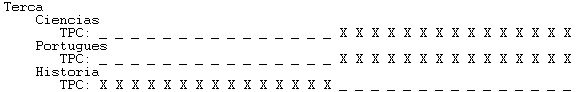
\includegraphics[width=1\textwidth]{tpc1}
\caption{Representação dos TPC's de uma disciplina}
\end{figure}

%PICTURE!
Este predicado é iterado várias vezes dependendo do número de turmas existentes.

Para o segundo predicado:
É iterada a solução por disciplina e é imprimida a disciplina, o conjunto de semanas em que existe teste e o(s) respetivo(s) dia(s) da semana, tal pode ser observado na imagem seguinte:
%Picture!
\begin{figure}
\centering
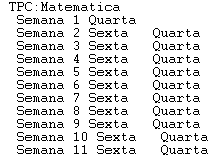
\includegraphics[]{tpc2}
\caption{Representação dos TPC's de uma disciplina}
\end{figure}

Explicar os predicados que permitem visualizar a solução em modo de texto

\section{Resultados}

\subsection{ Trabalhos de Casa}

Para comparação dos dois perdicados, foram executados para a mesma turma, cada turma possiu 5 disciplinas distintas, um número variável de semanas, com limite de 2 trabalhos de casa por dia. Seguem-se a seguir os resultados.

\begin{figure}
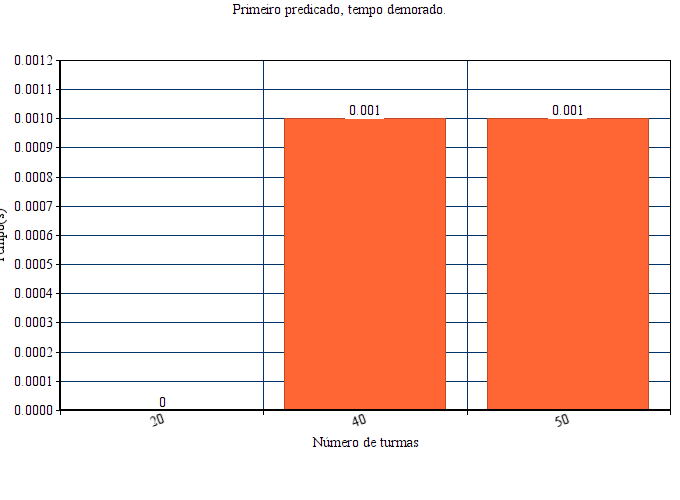
\includegraphics[width=0.5\textwidth]{g1}
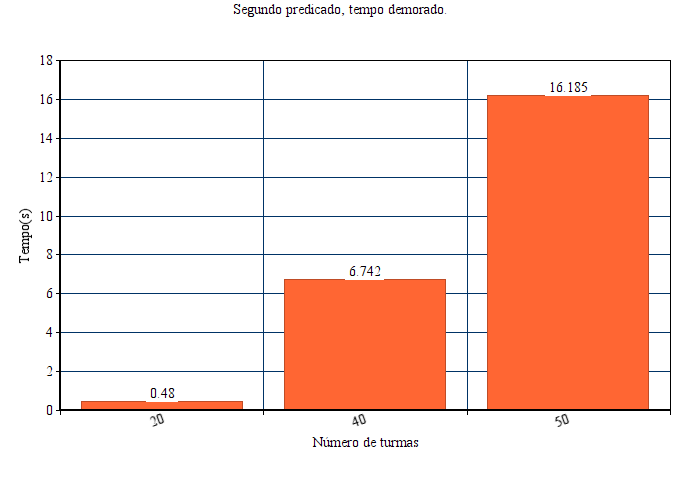
\includegraphics[width=0.5\textwidth]{g2}
\caption{Testes executados em ambos predicados}
\end{figure}

Como é possível obervar o primeiro predicado teve um tempo de execução muito superior ao segundo, isto deve-se ao facto do uso de variáveis de domínio binárias e também por não se preócupar com o número de ocorrências da disciplina ao longo da semana, já que apenas marca TPC's para metade das semanas de aula de uma disciplina de um determinado dia.
Em relação ao segundo predicado, por ter estas condições em conta e pelas variáveis não estarem instânciadas de forma binária, quanto maior o número de semanas, relfete-se o aumento exponencial do tempo.


\subsection{ Testes}

Demonstrar exemplos de aplicação em instâncias do problema com
diferentes complexidades e analisar os resultados obtidos. Devem ser utilizadas formas
convenientes para apresentação dos resultados (tabelas e/ou gráficos).

\section{Conclusões e Trabalho Futuro}
Este projeto premitiu esclarecer vários conceitos relacionados com a programação em lógica com restrições, foi possivél, para o grupo, obter uma visão mais detalhada sobre este paradigma assim como a sua importância na resolução de diferentes problemas de otimização/decisão. Também permitiu a precepção da importância da propagação das restrições de modo a melhorar o desempenho neste tipo de problemas.


Em relação aos trabalhos de casa:

Conclui-se que o primeiro predicado, devido à estrutura proposta para operar os dados foi possível otimizar a nivél de espaço o número de trabalhos de casa marcados, diminuindo consequentemente, o espaço de procura. A limitação trazida por esta estrutura é que, o plano escolar terá que ser tido em conta com semanas completas.  De modo a melhorar a especificação dos trabalhos de casa, poderão ser implementadas mais variáveis, de modo a fornecer mais flexibilidade no momento da pesquisa, como por exemplo, o dia livre ser variável de semana para semana, a utilização de listas de diferença de modo a melhorar o desempenho de como é feita a concatenação de listas, entre outros.

Conclui-se que o segundo predicado, devido à sua estrutura, foi capaz de minimizar o número de dias utilizados para marcar TPC's e foi possível a adaptação do predicado comulative, referênciado anteriormente. Em comparação com o primeiro predicado, utiliza uma estrutura muito mais flexivel, fácil de iterar, melhorias poderiam passar, por melhorar a procura do dia livre, esta procura é um fator importante no momento da pesquisa por soluções, um dia bem escolhido, já facilita bastante a marcação dos TPC's, a limitação realizada pelo grupo ainda é um bocado simplista, escolhendo os melhores dias para casos simples.


 Que conclusões retira deste projeto? O que mostram os resultados obtidos? Quais as vantagens e limitações da
solução proposta? Como poderia melhorar o trabalho desenvolvido



\begin{figure}
\vspace{2.5cm}
\caption{This is the caption of the figure displaying a white eagle and
a white horse on a snow field}
\end{figure}

\begin{table}
\caption{This is the example table taken out of {\it The
\TeX{}book,} p.\,246}
\begin{center}
\begin{tabular}{r@{\quad}rl}
\hline
\multicolumn{1}{l}{\rule{0pt}{12pt}
                   Year}&\multicolumn{2}{l}{World population}\\[2pt]
\hline\rule{0pt}{12pt}
8000 B.C.  &     5,000,000& \\
  50 A.D.  &   200,000,000& \\
1650 A.D.  &   500,000,000& \\
1945 A.D.  & 2,300,000,000& \\
1980 A.D.  & 4,400,000,000& \\[2pt]
\hline
\end{tabular}
\end{center}
\end{table}

\begin{equation}
\begin{array}{rcl}
  \dot{x}&=&JH' (x)\\
  x(0)&=&x (T)
\end{array}
\end{equation}


\begin{proposition}
Assume $H'(0)=0$ and $ H(0)=0$. Set:
\begin{equation}
  \delta := \liminf_{x\to 0} 2 N (x) \left\|x\right\|^{-2}\ .
  \label{eq:one}
\end{equation}

If $\gamma < - \lambda < \delta$,
the solution $\overline{u}$ is non-zero:
\begin{equation}
  \overline{x} (t) \ne 0\ \ \ \forall t\ .
\end{equation}
\end{proposition}


\paragraph{Notes and Comments.}
The results in this section are a
refined version of \cite{clar:eke};
the minimality result of Proposition
14 was the first of its kind.

To understand the nontriviality conditions, such as the one in formula
(\ref{eq:four}), one may think of a one-parameter family
$x_{T}$, $T\in \left(2\pi\omega^{-1}, 2\pi b_{\infty}^{-1}\right)$
of periodic solutions, $x_{T} (0) = x_{T} (T)$,
with $x_{T}$ going away to infinity when $T\to 2\pi \omega^{-1}$,
which is the period of the linearized system at 0.

%
% ---- Bibliography ----
%
\begin{thebibliography}{5}
%
\bibitem {url} 
SWI-Prolog,
\url{http://www.swi-prolog.org}
\bibitem {url} 
SICStus-Prolog,
\url{https://sicstus.sics.se}


\end{thebibliography}
\clearpage

\section*{Anexo}
\subsection*{Código fonte}

Bla Bla


\end{document}
